\documentclass{article}
\usepackage{graphicx}
\usepackage[utf8]{inputenc}
\usepackage{polski}
\usepackage{float}

\author{Kacper Haczkiewicz, Maria Kwintal, Laura Nowak, Paweł Nowak}
\title{\textbf{Projekt zaliczeniowy - dokumentacja}}
\date{Styczeń 2024}

\begin{document}
	
	\maketitle
	
	\section{Wstęp}
	
	Celem niniejszej dokumentacji jest szczegółowe przedstawienie komponentów projektu zaliczeniowego z przedmiotu Bazy Danych. Projekt dotyczy firmy Wombat Grylls sp. z o.o. organizującej wycieczki do miast, w których żyli znani matematycy. Dzięki niżej opisanej bazie danych możliwe jest przechowywanie i zarządzanie informacjami o miastach, klientach, pracownikach czy transakcjach związanych z firmą.
	
	Dokumentacja zawiera opis wykorzystanych technologii, strukturę plików, graficzny schemat bazy danych oraz szczegółowy opis tabel i relacji pomiędzy nimi. Uwzględniono również podsumowanie pracy nad projektem.
	
	\section{Spis użytych technologii}
	
	Do realizacji projektu użyto następujących technologii.
	\begin{enumerate}
		\item Python 3.12 - użyty do napisania skryptów generujących dane i wypełniających bazę. Projekt jest również kompatybilny z wersją 3.11.
		\item Biblioteki Pythona:
		\begin{itemize}
			\item Mysql.connector 9.1.0 - umożliwia komunikację między Pythonem a bazą danych MySQL.
			\item NumPy 2.1.3 - narzędzie do obliczeń numerycznych.
			\item Pandas 2.2.3 - biblioteka do manipulacji i analizy danych.
		\end{itemize}
		\item ERD Editor 2.0.4 - wykorzystany do stworzenia schematu bazy danych w formie diagramu ERD.
		\item R 4.4.2 - użyty do przygotowania raportu oraz analizy danych.
		\item Pakiety R:
		\begin{itemize}
			\item Dplyr - pakiet do manipulacji danych.
			\item Ggplot2 - narzędzie do tworzenia wizualizacji danych.
			\item KableExtra - używany do formatowania tabel.
			\item Knitr - pakiet do dynamicznego generowania raportów.
			\item Plotly - umożliwia tworzenie interaktywnych wykresów.
			\item RMariaDB - użyty do komunikacji z bazą danych MySQL w środowisku R.
		\end{itemize}
		\item LaTeX - użyty do przygotowania dokumentacji projektu.
	\end{enumerate}
	
	\section{Spis plików}
	
	Poniżej znajduje się opis plików zawartych w projekcie.
	\begin{enumerate}
		\item dokumentacja – katalog zawiera:
		\begin{itemize}
			\item dokumentacja.tex – kod źródłowy LaTeX, użyty do przygotowania dokumentacji projektu.
			\item dokumentacja.pdf - dokumentacja projektu w wersji PDF.
			\item diagram.PNG – graficzny schemat bazy danych.
		\end{itemize}
		\item generator\textunderscore danych.ipynb - skrypt Jupyter Notebook odpowiedzialny za generowanie danych. Dane te są zapisywane w katalogu Tabele\textunderscore csv.
		\item Imiona i nazwiska - katalog zawierający pliki CSV z danymi o popularnych imionach i nazwiskach, wykorzystywanymi przy generowaniu danych.
		\item raport.Rmd - zawierający kod źródłowy R, który generuje raport.
		\item schemat\textunderscore bazy.vuerd - plik zawiera schemat bazy danych w formacie ERD.
		\item Tabele\textunderscore csv - katalog zawierający wygenerowane wcześniej pliki csv z danymi, które wstawiane są następnie do bazy danych.
		\item Wstawiator\textunderscore danych.py - skrypt w Pythonie odpowiedzialny za wstawianie danych z katalogu Tabele\textunderscore csv do bazy danych.
		\item wycieczki.csv - plik zawierający informacje o rodzajach wycieczek czy kosztach biletów.
	\end{enumerate}
	
	\section{Kolejność i sposób uruchamiania plików}
	
	Do uruchomienia projektu należy posiadać niezbędny sprzęt (tj. komputer z systemem Windows z wersją przynajmniej 10 i dostępem do internetu). Należy również posiadać Python w wersji przynajmniej 3.11, R 4.4.2, LaTeX oraz dowolne środowiska programistyczne pozwalające na kompilację bądź interpretację powyższych plików.
	
	W celu uruchomienia projektu należy uruchomić następujące pliki w podanej kolejności.
	
	\begin{enumerate}
		\item generator\textunderscore danych.ipynb
		\item Wstawiator\textunderscore danych.py
		\item raport.Rmd
	\end{enumerate}
	
	\section{Schemat bazy danych}
	
	\subsection{Graficzny schemat bazy}
	
	Poniżej znajduje się graficzny schemat bazy danych.
	
	\begin{figure}[H]
		\centering
		\makebox[\textwidth][c]{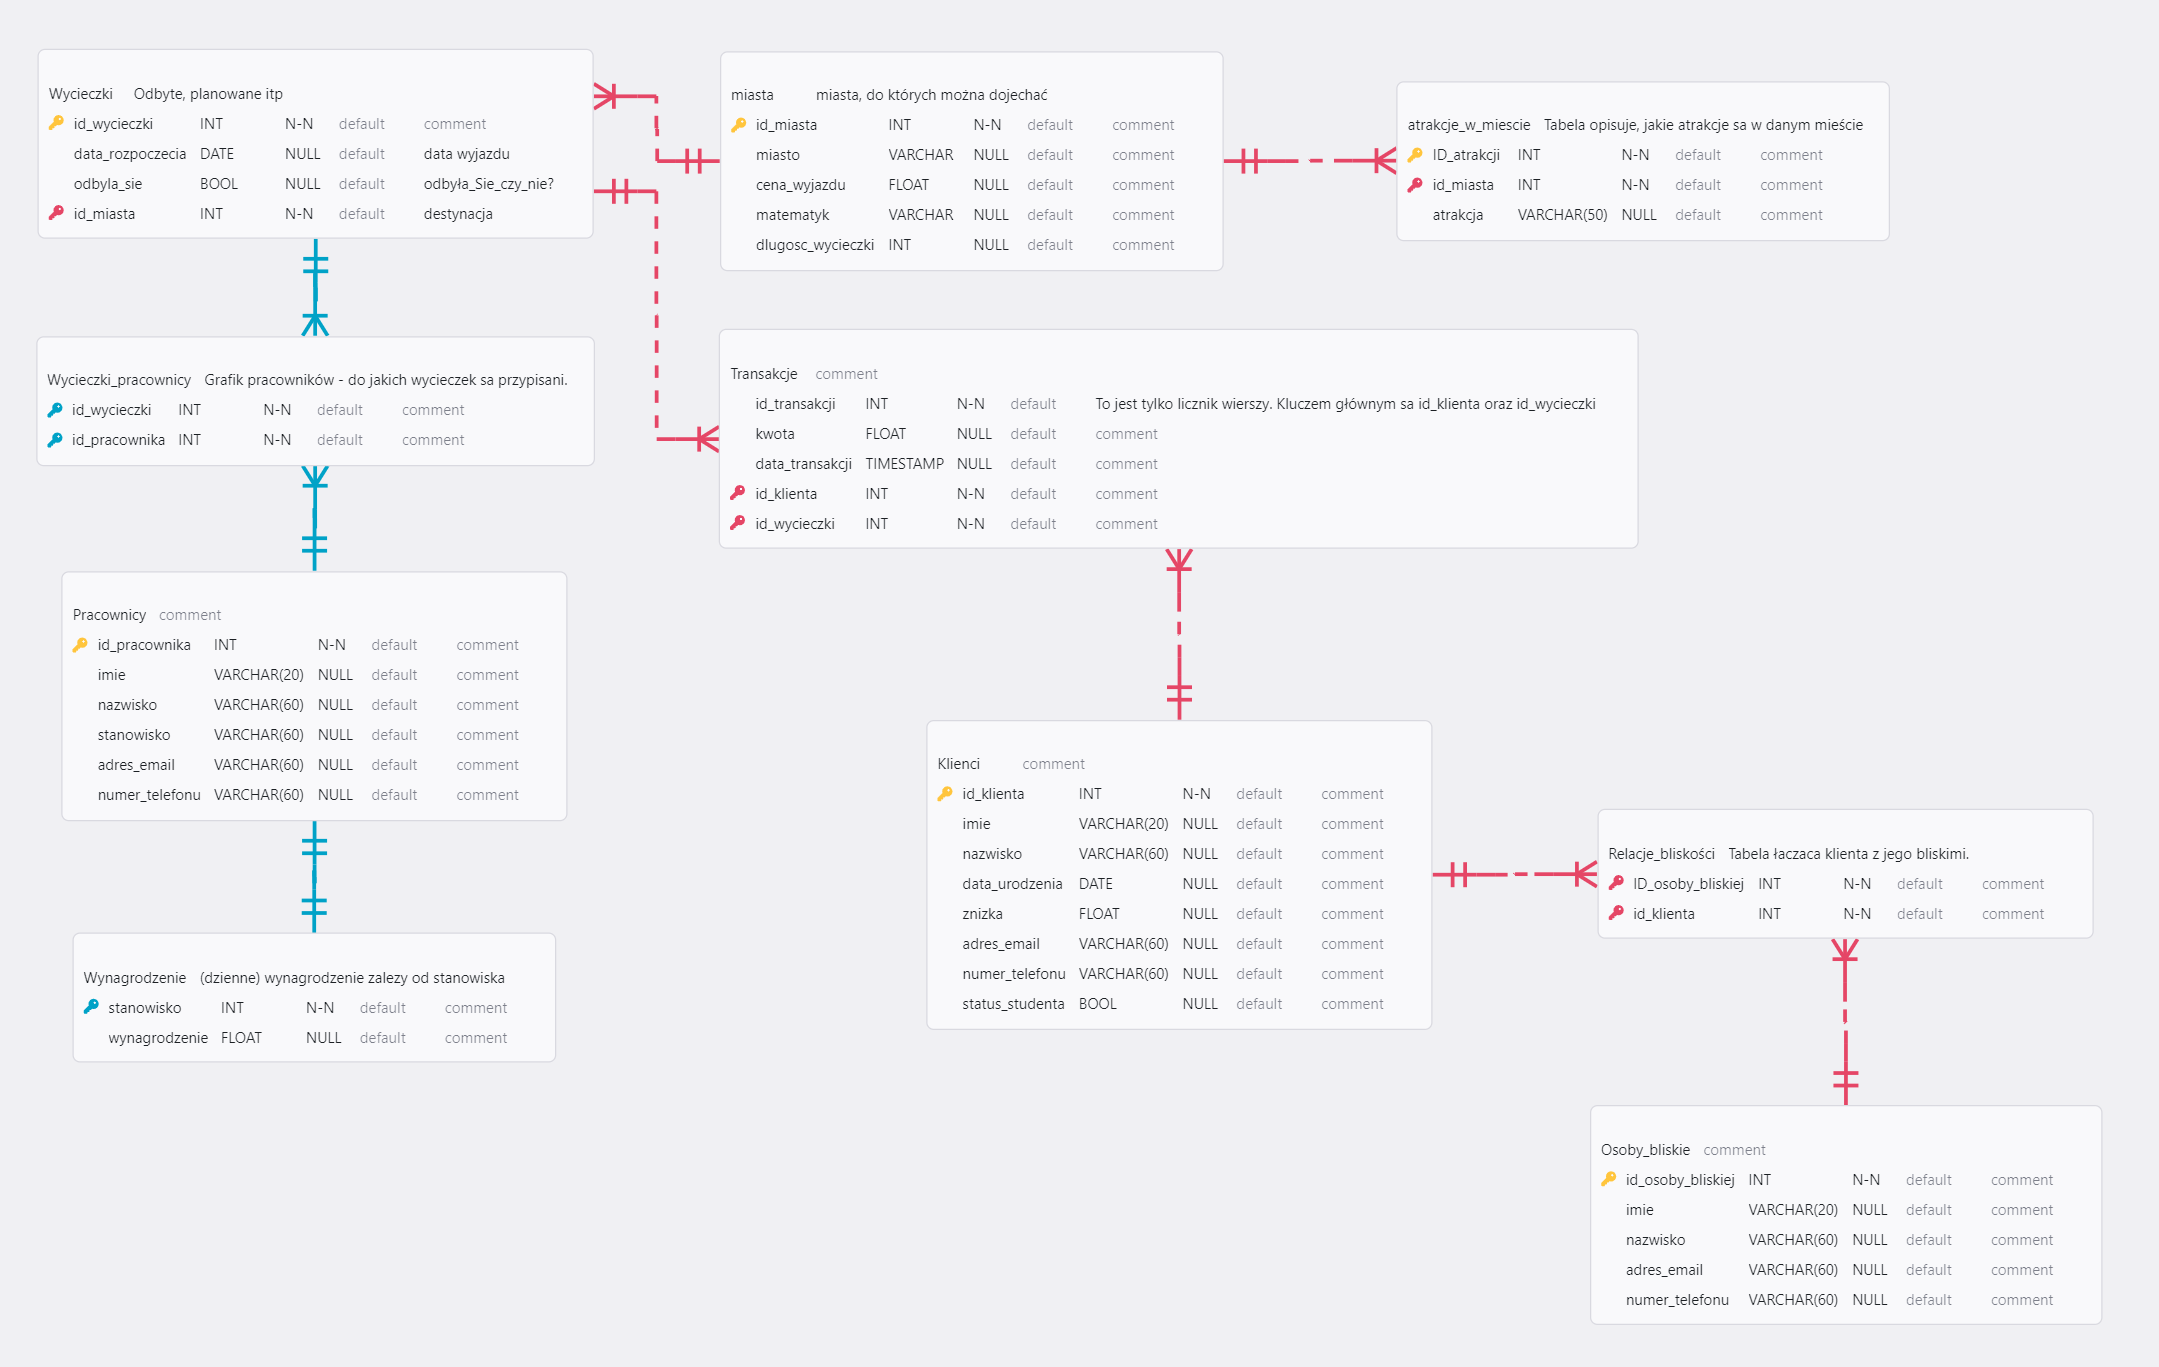
\includegraphics[width=1.3\textwidth]{diagram.PNG}}%
		\caption{Schemat bazy}
	\end{figure}
	
	\subsection{Opis tabel}
	
	Baza danych składa się z poniższych tabel. 
	
	\begin{enumerate}
		
		\item Atrakcje\textunderscore w\textunderscore miescie
		\begin{itemize}
			\item Atrybuty: id\textunderscore atrakcji (klucz główny), atrakcja, id\textunderscore miasta (klucz obcy).
			\item Zależności funkcyjne: id\textunderscore atrakcji → atrakcja, id\textunderscore miasta.
		\end{itemize}
		
		\item Klienci
		\begin{itemize}
			\item Atrybuty: id\textunderscore klienta (klucz główny), imie, nazwisko, data\textunderscore urodzenia, znizka, adres\textunderscore email, numer\textunderscore telefonu, status\textunderscore studenta.
			\item Zależności funkcyjne: id\textunderscore klienta → imie, nazwisko, data\textunderscore urodzenia, znizka, adres\textunderscore email, numer\textunderscore telefonu, status\textunderscore studenta.
		\end{itemize}
		
		\item Miasta
		\begin{itemize}
			\item Atrybuty: id\textunderscore miasta (klucz główny), miasto, cena\textunderscore wyjazdu, matematyk, dlugosc\textunderscore wycieczki.
			\item Zależności funkcyjne: id\textunderscore miasta → miasto, cena\textunderscore wyjazdu, matematyk, dlugosc\textunderscore wycieczki.
		\end{itemize}
		
		\item Osoby\textunderscore bliskie
		\begin{itemize}
			\item Atrybuty: id\textunderscore osoby\textunderscore bliskiej (klucz główny), imie, nazwisko, adres\textunderscore email, numer\textunderscore telefonu.
			\item Zależności funkcyjne: id\textunderscore osoby\textunderscore bliskiej → imie, nazwisko, adres\textunderscore email, numer\textunderscore telefonu.
		\end{itemize}
		
		\item Pracownicy
		\begin{itemize}
			\item Atrybuty: id\textunderscore pracownika (klucz główny), imie, nazwisko, stanowisko (klucz obcy), adres\textunderscore email, numer\textunderscore telefonu.
			\item Zależności funkcyjne: id\textunderscore pracownika → imie, nazwisko, stanowisko (klucz obcy), adres\textunderscore email, numer\textunderscore telefonu.
		\end{itemize}
		
		\item Relacje\textunderscore bliskosci
		\begin{itemize}
			\item Atrybuty: id\textunderscore osoby\textunderscore bliskiej (część klucza głównego), id\textunderscore klienta (część klucza głównego).
		\end{itemize}
		
		\item Transakcje
		\begin{itemize}
			\item Atrybuty: id\textunderscore transakcji (klucz główny), kwota, data\textunderscore transakcji, id\textunderscore klienta (klucz obcy), id\textunderscore wycieczki (klucz obcy).
			\item Zależności funkcyjne: id\textunderscore transakcji → kwota, data\textunderscore transakcji, id\textunderscore klienta (klucz obcy), id\textunderscore wycieczki (klucz obcy).
		\end{itemize}
		
		\item Wycieczki
		\begin{itemize}
			\item Atrybuty: id\textunderscore wycieczki (klucz główny), data\textunderscore rozpoczecia, odbyla\textunderscore sie, id\textunderscore miasta (klucz obcy).
			\item Zależności funkcyjne: id\textunderscore wycieczki → data\textunderscore rozpoczecia, odbyla\textunderscore sie, id\textunderscore miasta (klucz obcy).
		\end{itemize}
		
		\item Wycieczki\textunderscore pracownicy
		\begin{itemize}
			\item Atrybuty: id\textunderscore wycieczki (część klucza głównego, klucz obcy), id\textunderscore pracownika (część klucza głównego, klucz obcy).
		\end{itemize}
		
		\item Wynagrodzenie
		\begin{itemize}
			\item Atrybuty: stanowisko (klucz główny), wynagrodzenie.
			\item Zależności funkcyjne: stanowisko → wynagrodzenie.
		\end{itemize}
		
	\end{enumerate}
	
	\subsection{Opis relacji między tabelami}
	
	Pomiędzy tabelami występują następujące relacje.
	
	\begin{enumerate}
		
		\item Wycieczki i Wycieczki\textunderscore pracownicy
		\begin{itemize}
			\item Relacja 1:n - jeden pracownik może być przypisany do wielu wycieczek.
			\item Klucz główny tabeli Wycieczki (id\textunderscore wycieczki) występuje jako część klucza głównego w tabeli Wycieczki\textunderscore pracownicy.
		\end{itemize}
		 
		\item Wycieczki\textunderscore pracownicy i Pracownicy
		\begin{itemize}
			\item Relacja 1:n - jedna wycieczka może mieć wielu pracowników.
			\item Klucz główny tabeli Pracownicy (id\textunderscore pracownika) występuje jako część klucza głównego w tabeli Wycieczki\textunderscore pracownicy.
		\end{itemize}
	
		\item Pracownicy i Wynagrodzenie
		\begin{itemize}
			\item Relacja 1:1 - jeden pracownik może mieć jedno wynagrodzenie.
			\item Klucz główny tabeli Wynagrodzenie (stanowisko) występuje jako klucz obcy w tabeli Pracownicy.
		\end{itemize}

		\item Wycieczki i Miasta
		\begin{itemize}
			\item Relacja 1:n - wiele wycieczek może odbywać się w jednym mieście.
			\item Klucz główny tabeli Miasta (id\textunderscore miasta) jest kluczem obcym w tabeli Wycieczki.
		\end{itemize}
		
		\item Miasta i Atrakcje\textunderscore w\textunderscore miescie
		\begin{itemize}
			\item Relacja 1:n - w jednym mieście może być wiele atrakcji.
			\item Klucz główny tabeli Miasta (id\textunderscore miasta) jest kluczem obcym w tabeli Atrakcje\textunderscore w\textunderscore miescie.
		\end{itemize}
		
		\item Wycieczki i Transakcje
		\begin{itemize}
			\item Relacja 1:n - jedna wycieczka może być związana z wieloma transakcjami.
			\item Klucz główny tabeli Wycieczki (id\textunderscore wycieczki) występuje jako klucz obcy w tabeli Transakcje.
		\end{itemize}
		
		\item Transakcje i Klienci
		\begin{itemize}
			\item Relacja 1:n - jeden klient może być związany z wieloma transakcjami.
			\item Klucz główny tabeli Klienci (id\textunderscore klienta) występuje jako klucz obcy w tabeli Transakcje.
		\end{itemize}
		
		\item Klienci i Relacje\textunderscore bliskosci
		\begin{itemize}
			\item Relacja 1:n - jeden klient może mieć wiele przypisanych relacji z osobami bliskimi.
			\item Klucz główny tabeli Klienci (id\textunderscore klienta) występuje jako klucz obcy w tabeli Relacje\textunderscore bliskosci.
		\end{itemize}
		
		\item Relacje\textunderscore bliskosci i Osoby\textunderscore bliskie: 
		\begin{itemize}
			\item Relacja 1:n - jedna osoba bliska może być powiązana z wieloma klientami.
			\item Klucz główny tabeli Osoby\textunderscore bliskie (id\textunderscore osoby\textunderscore bliskiej) występuje jako klucz obcy w tabeli Relacje\textunderscore bliskosci.
		\end{itemize}
		 
	\end{enumerate}
	
	\subsection{Uzasadnienie, że baza jest w EKNF}
	
	Baza danych spełnia założenia EKNF, ponieważ:
	\begin{enumerate}
		\item Dane przechowywane w tabelach są atomowe, a wiersze nie są powielone (czyli spełnia 1NF).
		\item Wyeliminowano wszystkie częściowe zależności od jakiegokolwiek klucza potencjalnego (czyli spełnia 2NF).
		\item Wszystkie atrybuty niekluczowe są zależne tylko i wyłącznie od klucza głównego, a nie od innych atrybutów niekluczowych (czyli spełnia 3NF).
		\item Każda nietrywialna zależność funkcyjna ma postać, w której lewa strona jest nadkluczem lub prawa strona zawiera atrybut elementarny (czyli spełnia EKNF).
	\end{enumerate}
	
	Zatem baza danych jest w EKNF.
	
	\section{Podsumowanie projektu}
	
	Podczas realizacji projektu wyzwaniem okazało się zaplanowanie i przygotowanie schematu bazy danych. Był to kluczowy etap pracy nad projektem, ponieważ na nim opierała się reszta jego realizacji. Wymagające było również generowanie danych. Proces ten okazał się czasochłonny i wymagał zaawansowanej wiedzy z zakresu pisania skomplikowanych skryptów w Pythonie.
	
	Pomimo różnych trudności projekt pozwolił nam znacząco rozwinąć umiejętności z zakresu pracy z bazami danych. Ponadto pozwolił nam rozwinąć się w pracy zespołowej, szczególnie w rozdzielaniu zadań oraz efektywnej współpracy. To doświadczenie może okazać się przydatne w przyszłej pracy zawodowej.
	
\end{document}